\section{plugin.h File Reference}
\label{plugin_8h}\index{plugin.h@{plugin.h}}




This graph shows which files directly or indirectly include this file:\begin{figure}[H]
\begin{center}
\leavevmode
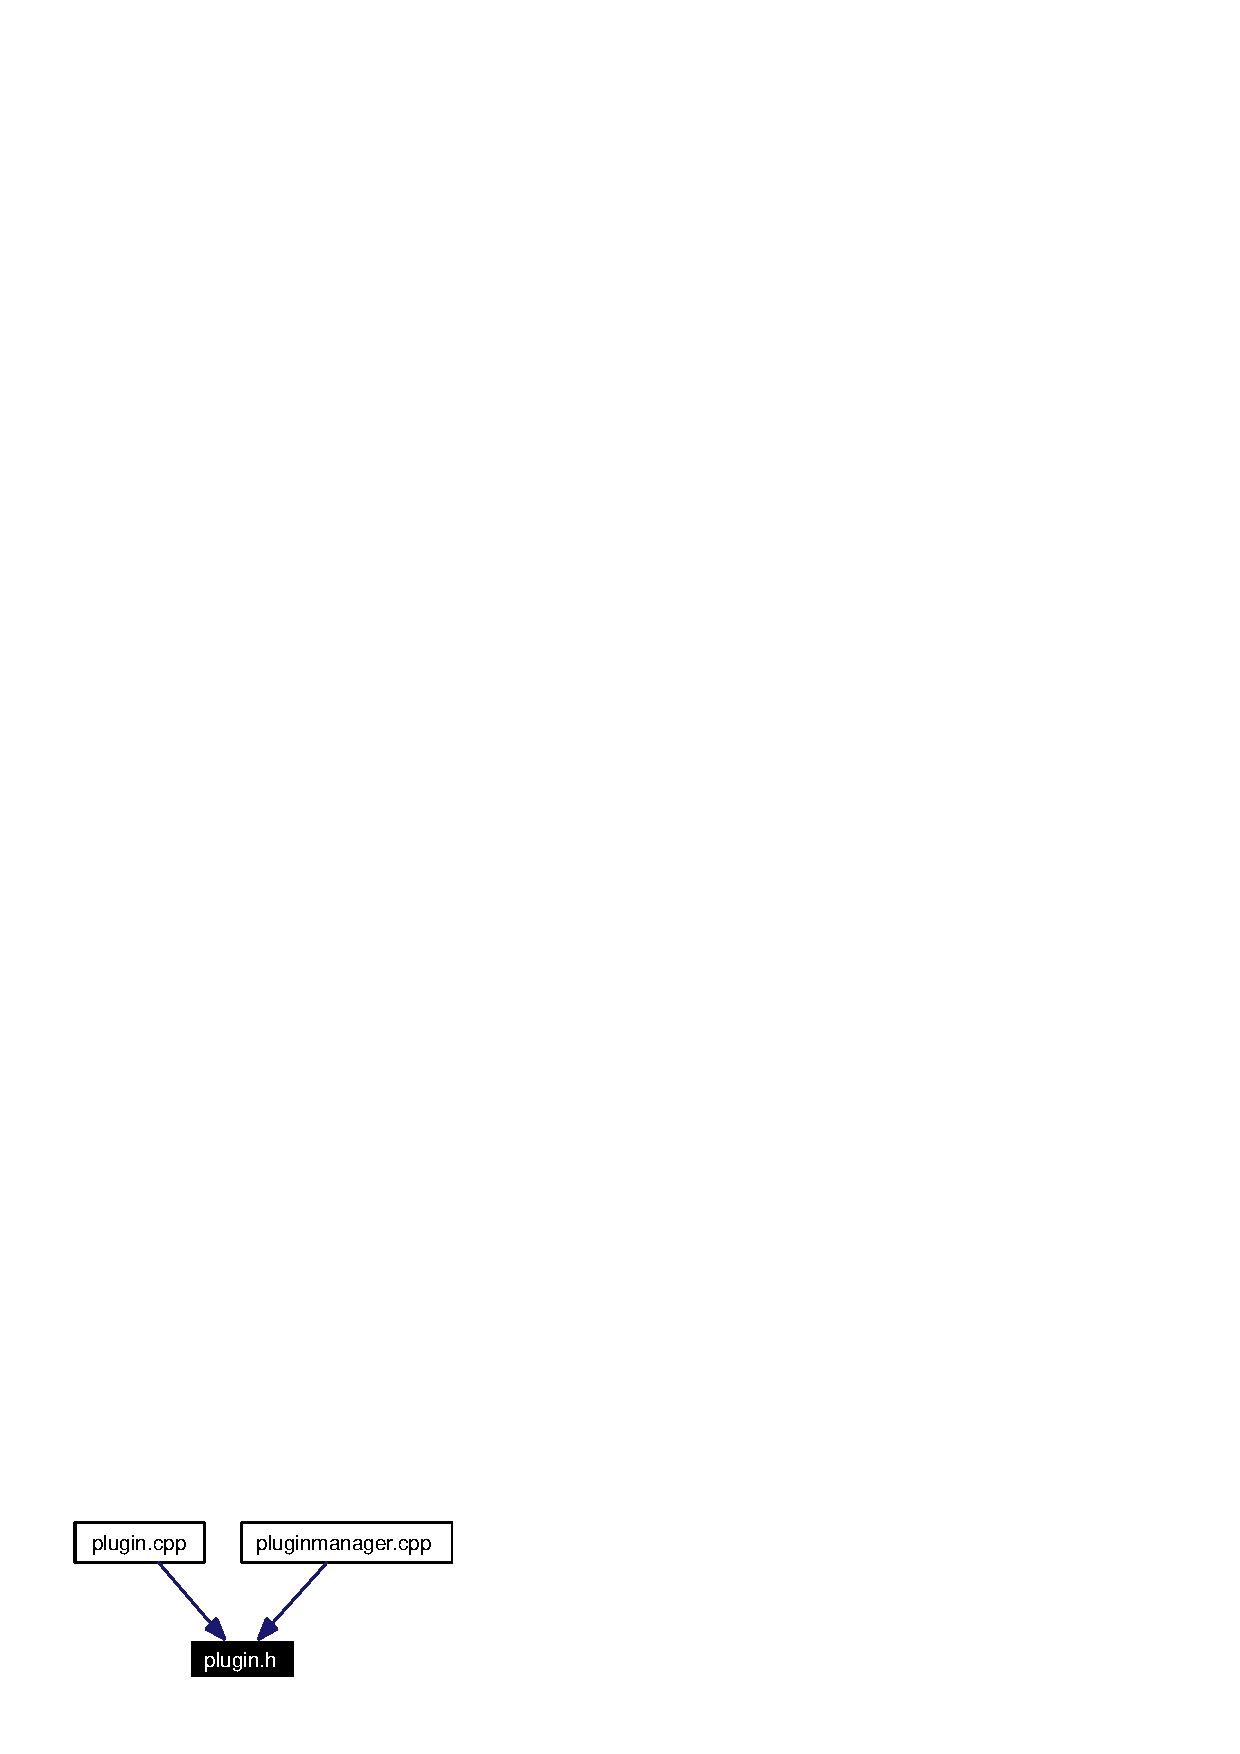
\includegraphics[width=108pt]{plugin_8h__dep__incl}
\end{center}
\end{figure}
\subsection*{Classes}
\begin{CompactItemize}
\item 
class {\bf Plugin}
\end{CompactItemize}
\subsection*{Defines}
\begin{CompactItemize}
\item 
\#define {\bf AMAROK\_\-EXPORT\_\-PLUGIN}(classname)
\end{CompactItemize}


\subsection{Define Documentation}
\index{plugin.h@{plugin.h}!AMAROK_EXPORT_PLUGIN@{AMAROK\_\-EXPORT\_\-PLUGIN}}
\index{AMAROK_EXPORT_PLUGIN@{AMAROK\_\-EXPORT\_\-PLUGIN}!plugin.h@{plugin.h}}
\subsubsection{\setlength{\rightskip}{0pt plus 5cm}\#define AMAROK\_\-EXPORT\_\-PLUGIN(classname)}\label{plugin_8h_a0}


{\bf Value:}

\footnotesize\begin{verbatim}extern "C" { \
         amaroK::Plugin* create_plugin() { return new classname; } \
    }
\end{verbatim}\normalsize 
Size doesn't matter! 

Definition at line 14 of file plugin.h.